\chapter{主机属性识别系统的设计与实现}

为了可以从实时网络中进行大规模的细粒度主机属性识别,本章基于前文的研究成果,设计并实现了一套原型系统,可在真实网络中较为准确地识别客户端主机的操作系统种类、版本以及浏览器种类等属性,并具备网络协议识别与解析、TLS流数据属性标注、日志信息存储与查询、主机属性发现实时可视化等功能。本章首先介绍系统的设计原则与目标,展示主机属性识别系统的组织架构、主要模块与功能。然后详细介绍各个模块的具体实现和关键算法。最终在开放网络中部署完整的原型系统,并从多个角度测试系统效果与性能。

\section{设计原则与目标}

在原型系统设计之前,为了更高效率的开发,本章提出了五项设计原则作为指导,分别是准确率高,隐蔽性强,识别范围广,处理速度快,结果可存储、查询和分析等。
\begin{itemize}

\item
准确率高。主机属性识别作为网络攻防的首要任务,识别的准确率、精度和召回率等指标关系着后续步骤的实施效果,决定了整个攻防任务的成败,是设计目标中的重中之重。
\item
隐蔽性强。在识别过程中应避免引起检测对象的察觉,由于本文采用被动识别方法,只需利用网络嗅探技术从网络节点中捕获流量,本身的隐蔽性能已经满足需求。
\item
识别范围广。传统主机属性识别方法多依赖于指纹库匹配,对于匹配失败的未知指纹无法进行有效识别。原型系统应摒弃指纹库的搭建,利用机器学习模型学习主机指纹的样本空间,具备较强的灵活性。
\item
处理速度快。原型系统将部署在大规模的网络中,必须具备适应高速流量的吞吐量。
\item
结果可存储、查询和分析。在对大规模网络中的主机属性进行识别后,预测结果可以保存在数据库中,并且利用可视化技术向用户提供图形界面,完成识别结果的简单分析。
\end{itemize}

\section{原型系统的组织架构}

本原型系统由五部分模块组成,包括流量采集模块、特征提取模块、属性识别模块、分类器更新模块以及数据存储与可视化模块。系统的组织结构如图5.1所示。

\begin{figure}[!h]
    \centering
    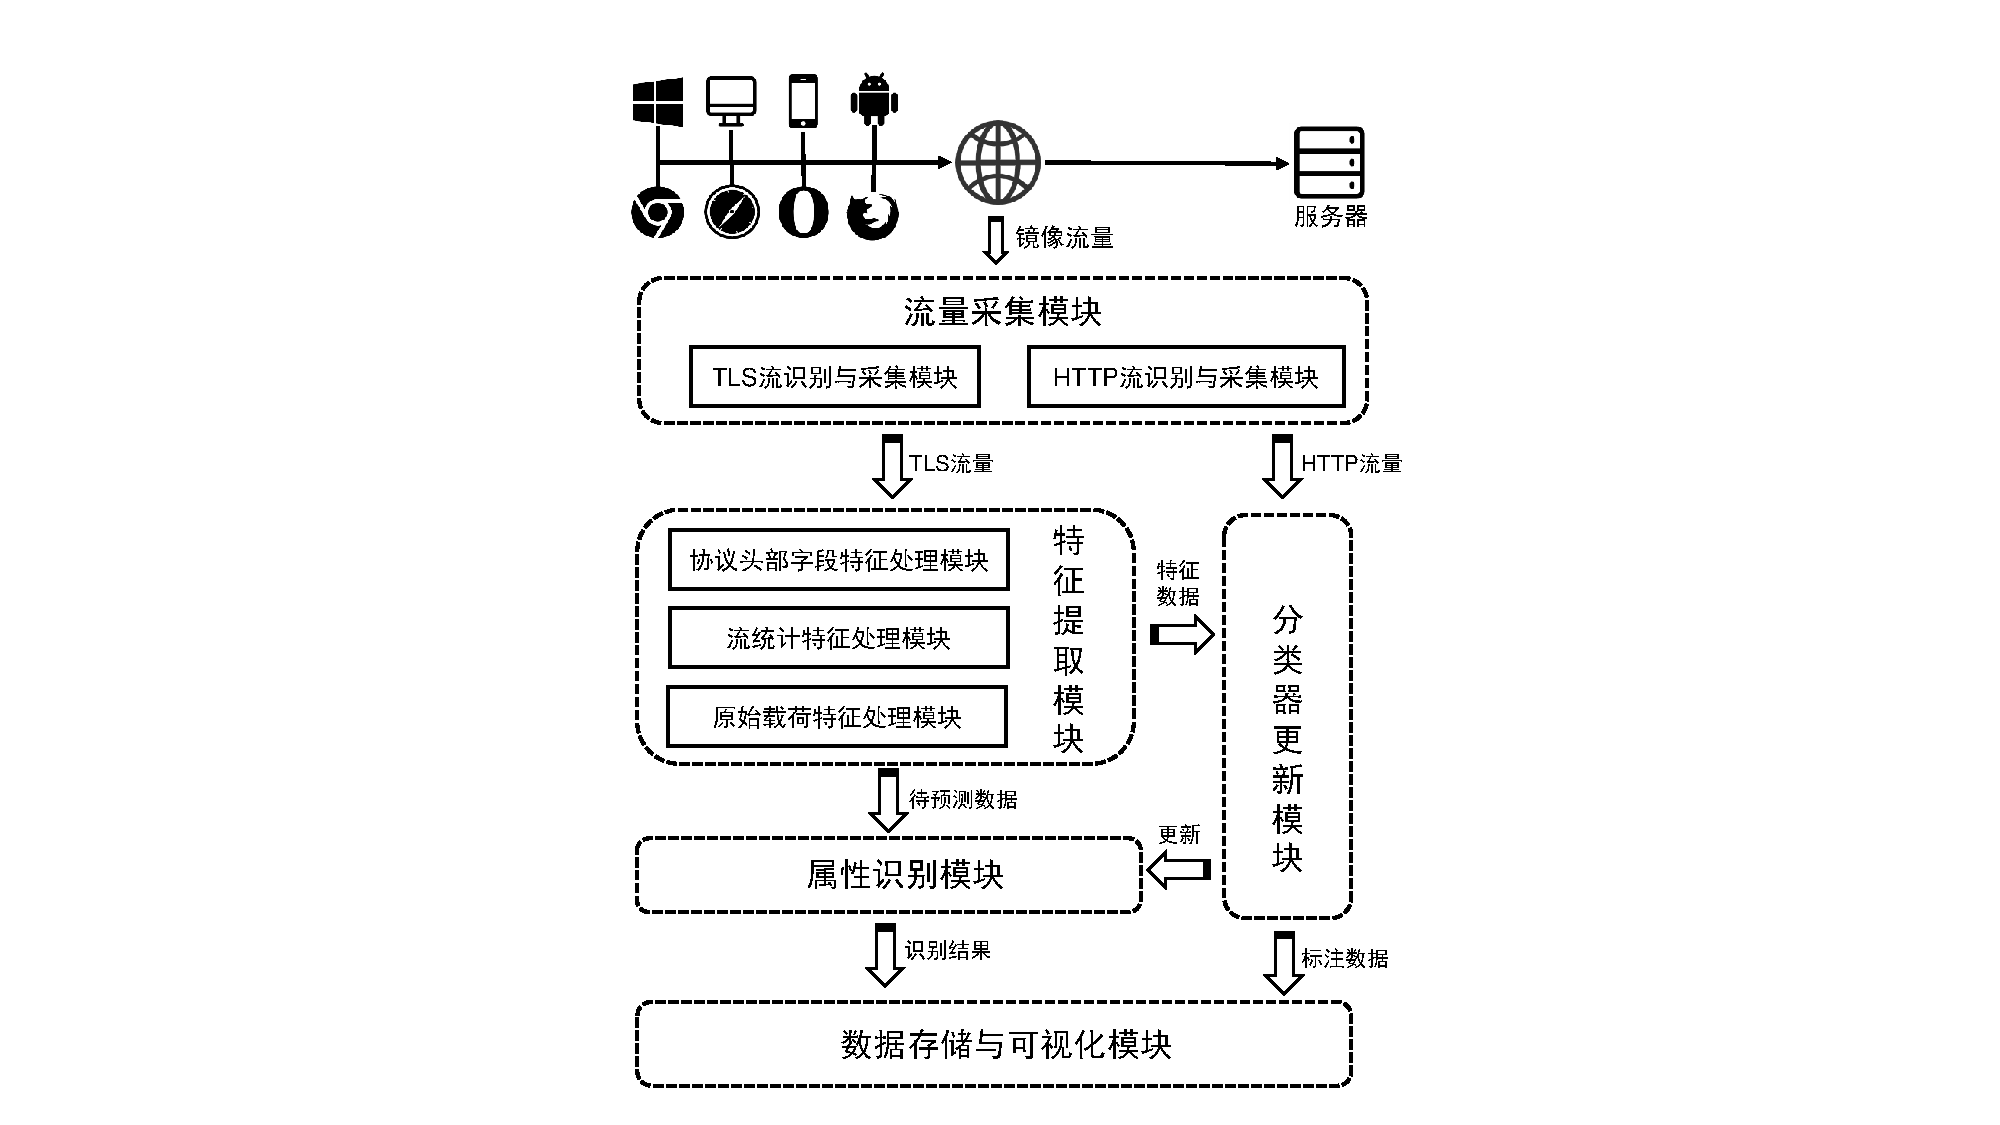
\includegraphics[width=0.7\textwidth]{原型系统架构}
    \bicaption{系统的组织架构}{Organizational structure of the system}
    \label{fig:5-1}
\end{figure}

流量采集模块:从实时网络中识别目标协议网络会话,并将同一会话的所有报文按序汇聚为双向流。

特征提取模块:对网络流数据进行格式解析,提取所需协议首部字段特征,统计网络流前50个数据包的长度序列特征和时间序列特征,对此类人工特征进行数据预处理后传递给属性识别模块中的集成树模型。此外,拼接TCP SYN包和TLS Client Hello包的原始字节数据并进行归一化处理,然后传递给属性识别模块中的神经网络模型进行属性预测。

属性识别模块:为了综合统计机器学习模型和深度学习模型的优点,利用Stacking技术将多个集成树模型和神经网络模型进行融合,进一步提升识别效果。

分类器更新模块:由于训练后的分类器只能识别已知的主机属性类型,为了增强系统的可扩展性,分类器更新模块可以从客户端的HTTP请求中解析出客户端主机信息,并将之与同一客户端的TLS流进行关联,构造有标签的训练数据集。并结合已有的数据集,对属性识别模块中的第一层模型进行离线训练,使得更新后的模型可识别更多的主机属性类别。

数据存储与可视化模块:首先利用Logstash数据采集引擎收集属性识别模块产生的结果日志,然后将Elasticsearch作为数据库和检索工具,最后使用Kibana工具从结果数据中生成Web界面,完成可视化功能。

本系统的工作流程是先由流量采集模块从目标网络中被动收集镜像流量,以双向流为单位给其他模块提供原始数据来源。特征提取模块通过解析获取的TLS流数据,得到协议字段特征、流统计特征以及原始字节数据,在经过数据预处理和特征转换后,为其他模块提供特征数据来源。属性识别模块和分类器更新模块分别基于特征数据进行预测和训练,同时离线训练模块中的模型可以根据需要为属性识别模块中的模型提供更新。最终,属性识别模块的预测结果由数据存储与可视化模块进行存储、查询与可视化。

\section{流量采集模块}

流量采集模块主要负责从网络中识别和采集HTTP流量和TLS流量,模块内结构如图5.2所示。按照RFC文档规定,HTTP协议的服务端口一般为80端口,TLS协议的服务端口一般为443端口。因此,本模块首先基于端口识别目标流量,然后以五元组<客户端IP, 服务端IP, 客户端端口, 服务端端口,传输层协议类型>为单位将每个网络会话的数据包汇聚为双向流,同时记录每个数据包的捕获时间以形成包到达时间序列,再根据RFC文档中协议格式的定义对数据包进行解析,丢弃协议格式异常的网络流。最终,将过滤后的目标流量及其包到达时间序列传输到特征提取模块和分类器更新模块。

\begin{figure}[!h]
    \centering
    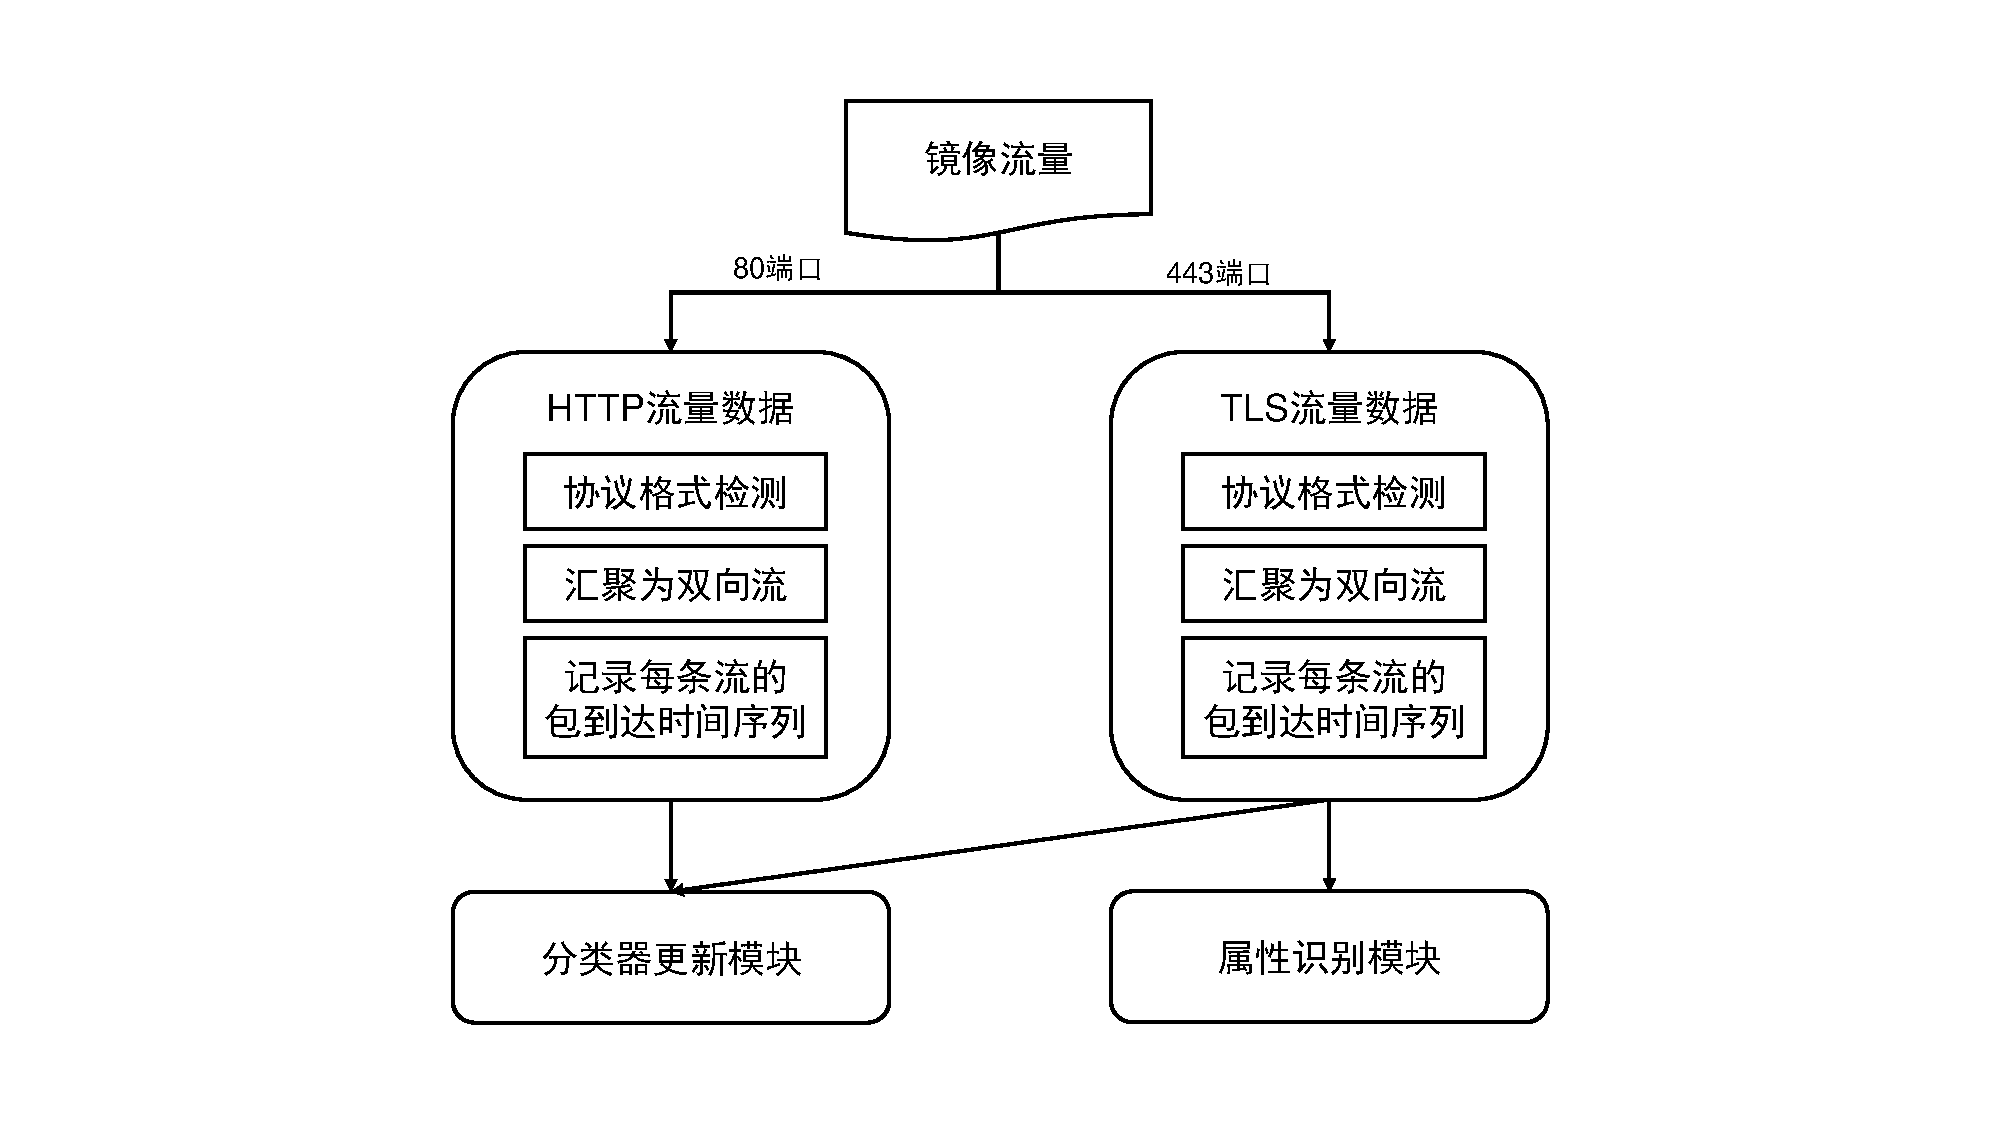
\includegraphics[width=0.6\textwidth]{流量采集模块}
    \bicaption{流量采集模块}{Traffic collection module}
    \label{fig:5-2}
\end{figure}

\section{特征提取模块}

在获取TLS流量后,特征提取模块根据协议格式标准对每条双向流的所有报文进行格式解析。当判定目标流量没有异常后,筛选出每条双向流地TCP SYN包和TLS Client Hello包以供接下来的各特征提取模块使用,其工作流程如图5.3所示。

\begin{figure}[!htbp]
    \centering
    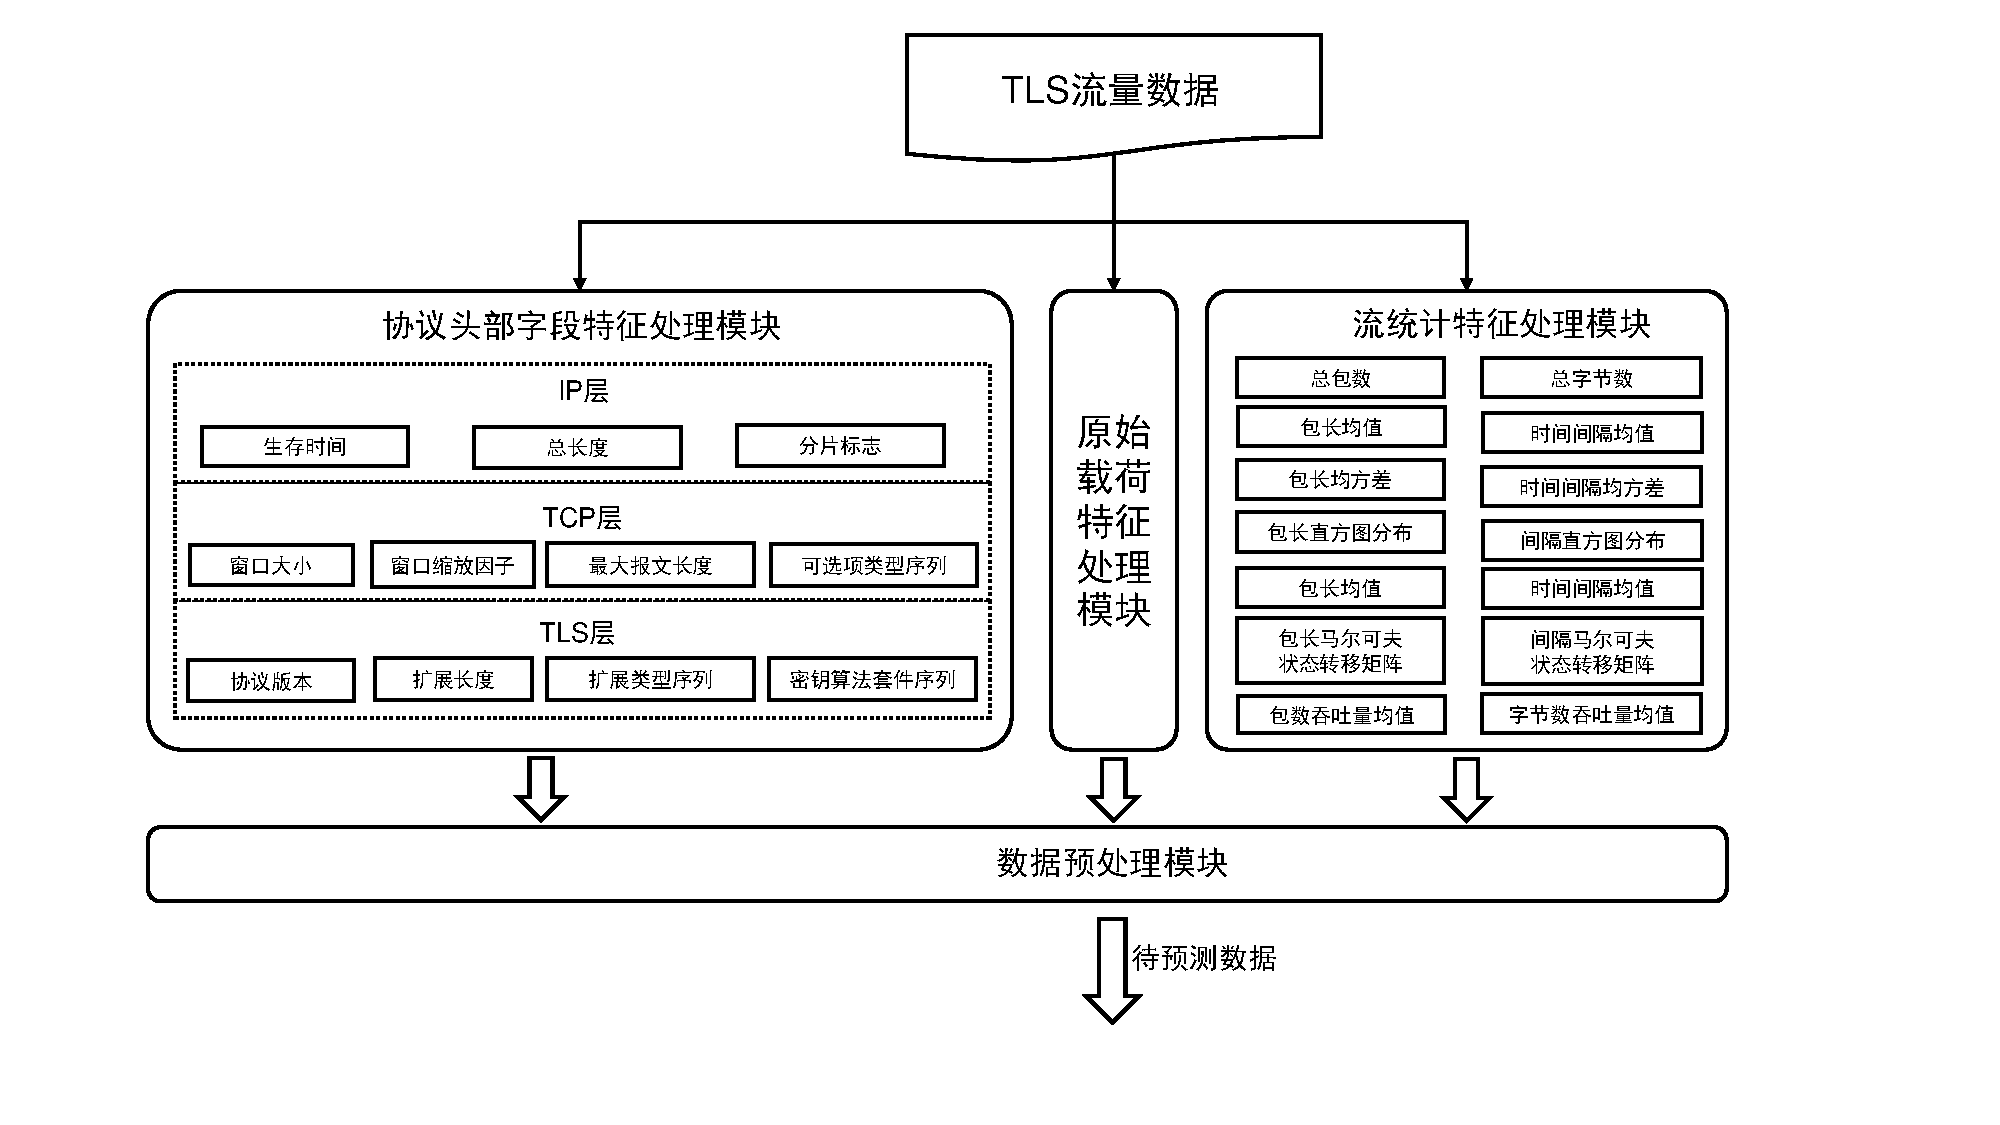
\includegraphics[width=0.9\textwidth]{特征提取模块}
    \bicaption{特征提取模块}{Feature extraction module}
    \label{fig:5-2}
\end{figure}

协议头部字段特征处理模块主要从TCP SYN包中提取IP协议首部的生存时间、总长度、分片标志等字段信息和TCP协议首部的窗口大小、窗口缩放因子、最大报文长度、可选项类型序列等字段信息,从TLS Client Hello包中提取协议版本、密钥算法套件序列、扩展长度、扩展类型序列、支持加密组件序列以及应用层协议协商状态码序列等字段信息。接着对于以上十三维特征进行各种数据预处理操作,包括缺失值填充,异常值处理,字符串特征编码等,得到可直接作为机器学习模型输入的十三维离散特征。

流统计特征处理模块的功能是提取和处理TLS流前50个包的包长序列特征和包到达时间序列特征。包长序列可由50个包的每包长度直接获取,通过计算便可得到包长均值、均方差、直方图分布和马尔可夫状态转移矩阵等统计特征。包到达时间序列由流量采集模块记录并提供,根据包到达时间序列可以计算得到包到达时间间隔均值、均方差、直方图分布和间隔马尔可夫状态转移矩阵等统计特征。最后通过统计完整流的所有报文信息,可得到总包数、总字节数、包数吞吐量均值、字节数吞吐量均值以及传输峰值分布等特征。对于以上连续特征进行数据归一化处理后,得到可作为机器学习模型输入的420维特征。

原始载荷特征处理模块的功能较为简单,主要从TCP SYN包中提取出IP层和TCP层的首部原始字节,从TLS Client Hello包中提取出TLS层的首部原始字节,对以上字节按序拼接在一起,并设置长度阈值为500字节,对长度大于500的原始字节序进行截断处理,对长度小于500的原始字节序进行填零补充。最终将长度为500的原始字节序进行归一化处理后,便可得到作为深度学习模型输入的500维特征。

\section{属性识别模块}

由于在实际的学习任务中,很难找到一个稳定性和预测性能都令人满意的模型,因此本系统的属性识别模块采用了双层结构的集成机器学习分类器。集成学习通过融合多个基模型,可以得到一个泛化性能更好的集成模型。在本模块中,第一层模型分别是以协议首部字段特征、流统计特征为输入的集成树模型和以原始字节序为输入的神经网络模型,第二层模型是以第一层模型预测结果为输入的逻辑回归模型。集成树模型包括3.3节中介绍的RF模型和LightGBM模型,神经网络模型包括4.2节中介绍的一维CNN模型和LSTM模型。

\begin{figure}[!h]
    \centering
    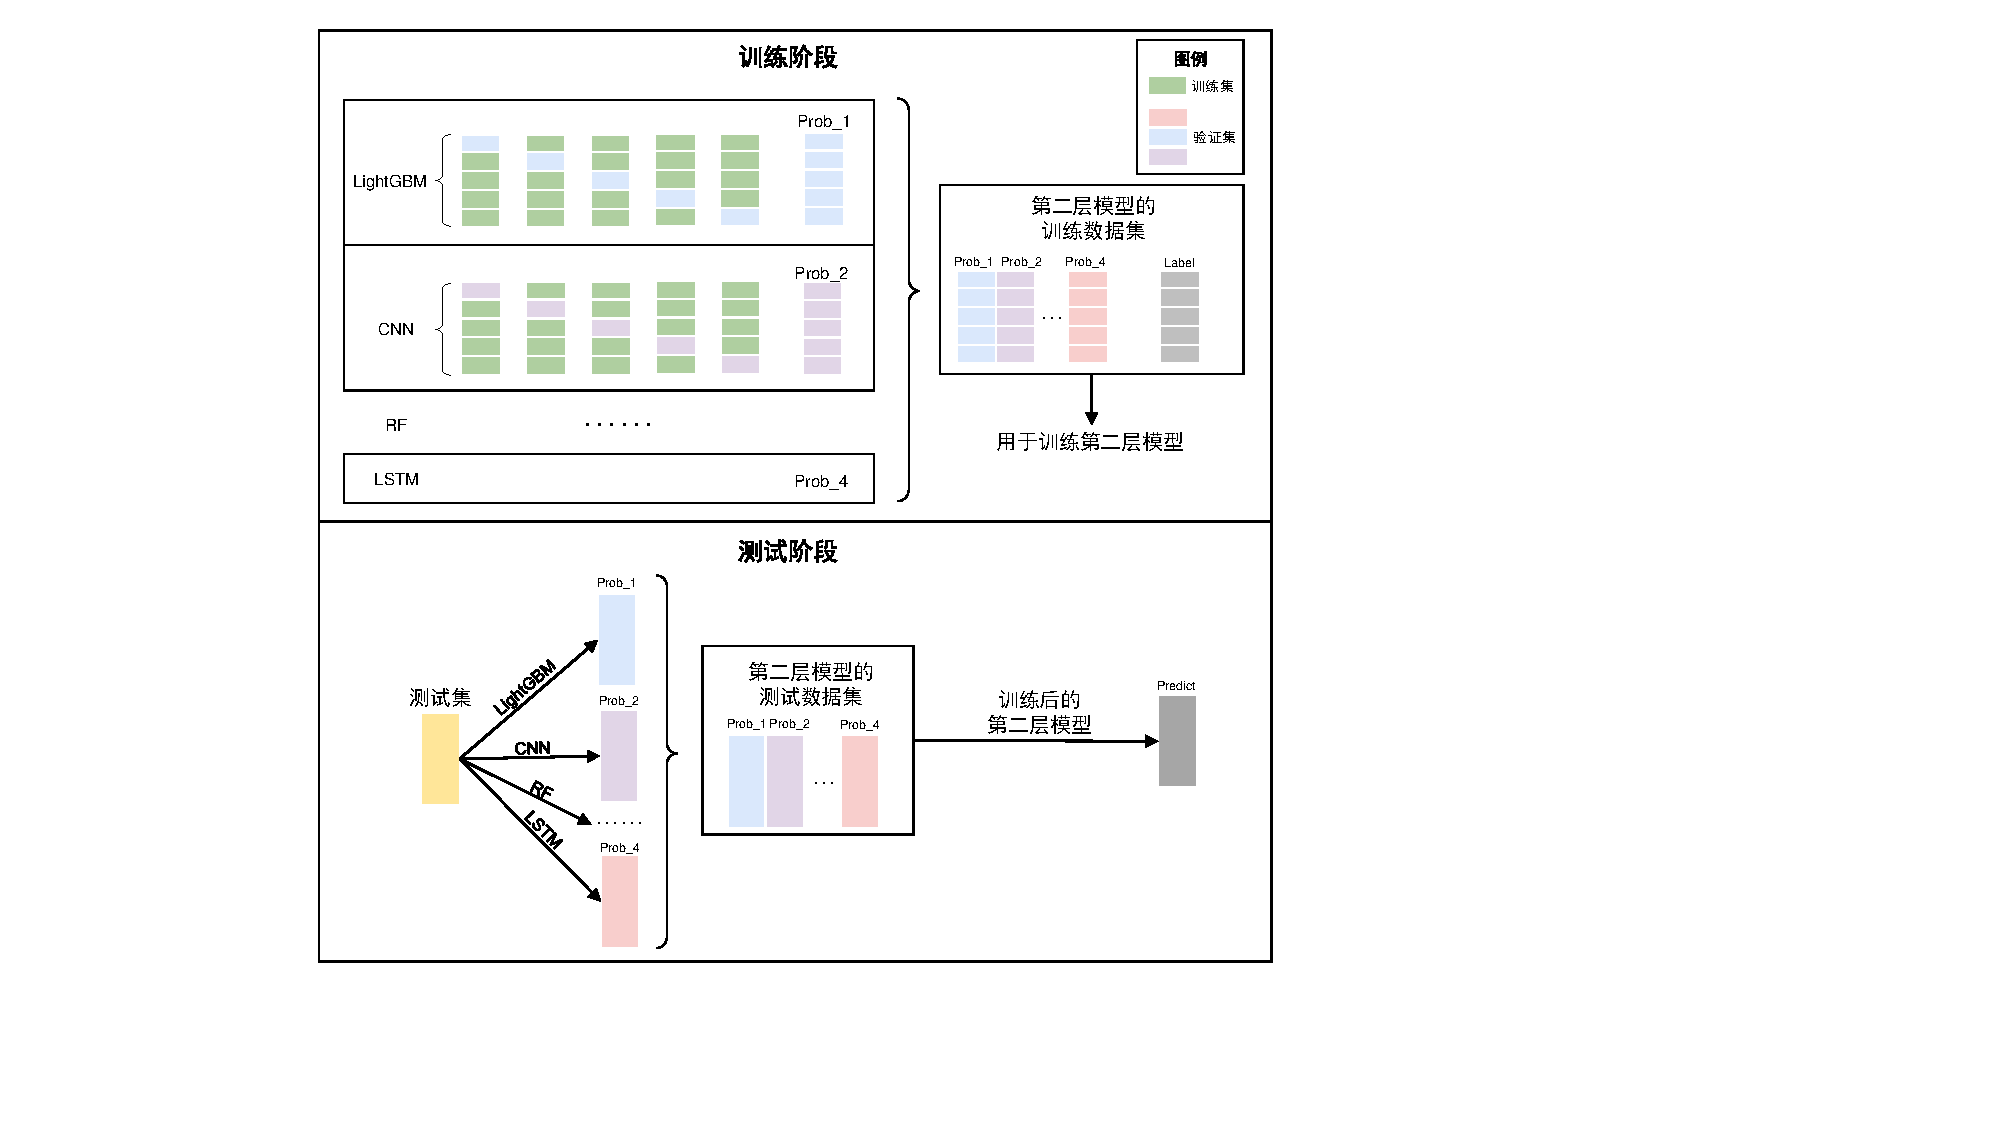
\includegraphics[width=0.9\textwidth]{stacking2}
    \bicaption{Stacking算法原理}{Stacking algorithm principle}
    \label{fig:5-3}
\end{figure}

本模块集成方法利用的主要思想是Stacking算法,和深度学习算法类似,Stacking算法也是一种表示学习算法,通过训练高层模型学习使用基模型的预测数据,可以实现对基模型的选择性表达,是目前提升机器学习效果最好的算法之一。Stacking算法原理如图5.4所示,在训练阶段中,首先利用K折交叉验证将原始训练集切分为K个子集,图中K值为5,然后将每个基模型训练并预测K次,每次训练循环以1个子集为验证集,以其余子集为训练集,最终得到四个模型在训练集上的类别预测概率数据,即为高层模型的训练特征数据。结合原始训练集中的标签数据,便可完成对高层模型的训练。

在测试阶段中,对于单个模型,利用其在K折交叉验证中的K次训练,可以对测试集数据进行预测K次,然后取这K次预测概率结果的均值,得到单个模型对测试集的类别预测概率数据。然后拼接所有基模型的预测概率数据,作为高层模型的预测特征数据。最后利用训练后的高层模型对特征数据进行预测,即可得到集成模型对测试集中所有样本的分类结果。
%将每个模型的预测结果拼接后得到Stacking训练集。同理,将K折交叉验证过程中每次训练后的基模型对原始测试集进行预测,最后取均值后得到Stacking测试集。在第二层模型中,通常选用原理和结构简单的机器学习模型从第一层的模型输出中学习有效特征,类似于投票器,本质是对第一层模型预测结果的权重学习。

%同其他集成学习方法一样,为了得到更强的泛化性能,进行Stacking集成时要求基学习器尽量保持独立,且效果相近。在3.4节的对比实验中可以看到,RF模型、XGBoost模型和LightGBM模型性能都比较优秀,但RF模型是基于Bagging算法,XGBoost模型和LightGBM模型都是基于Boosting算法,原理近似,因此本模块选择RF模型、LightGBM模型、一维卷积神经网络模型和长短期记忆网络模型等四种原理不同、性能优秀的模型作为基学习器。

属性识别模块利用以上介绍的集成分类器,可高效、精准地从样本数据中识别出每条加密流的客户端主机属性,目前主机属性包括操作系统种类、版本以及浏览器种类。未来可根据需求,结合分类器更新模块,扩展识别种类更多、粒度更细的主机属性。

\section{分类器更新模块}

分类器更新模块的功能是为属性识别模块中的分类器提供模型更新和优化服务,本质是对集成分类器的再训练过程,工作流程如图5.5所示。

\begin{figure}[!htbp]
    \centering
    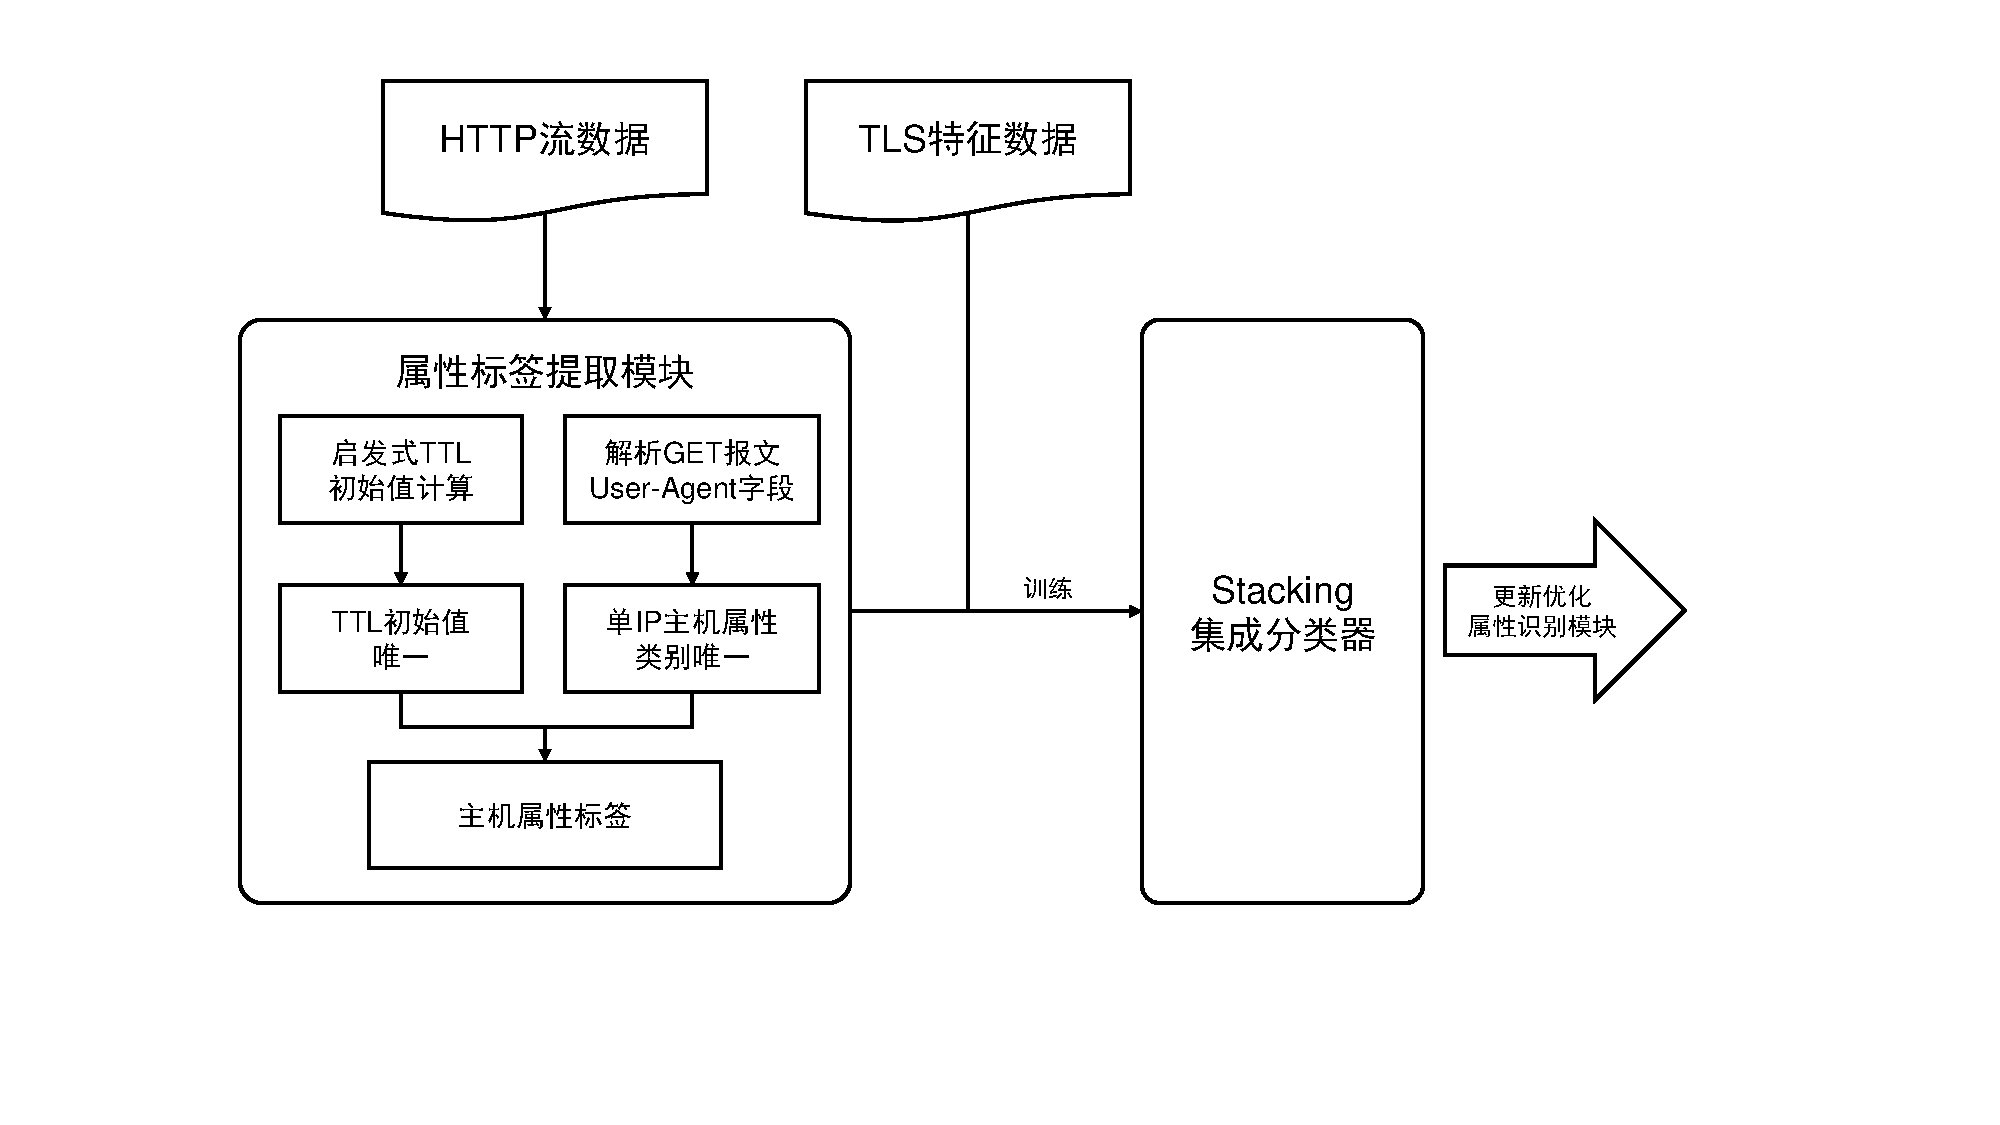
\includegraphics[width=0.9\textwidth]{5-4}
    \bicaption{分类器更新模块}{Classifier update module}
    \label{fig:5-4}
\end{figure}

由于考虑到系统的可扩展性,即在未来的主机属性发现场景中可能需要识别更多类别的操作系统和浏览器,分类器更新模块基于3.4节中介绍的属性标注方法,可以从HTTP流数据和TLS特征数据中构造有标签的数据集。然后分类器更新模块利用该数据集对Stacking集成模型进行离线训练,不会影响系统的实时识别功能。当离线模型的识别性能满足要求时,停止训练并将训练好的模型替换到属性识别模块中,完成对分类器的更新过程。

%由于本文中分类器的训练属于监督学习,必须基于有标签的数据集。而流量采集模块从网络中提取出的TLS流信息只包含训练任务所需的特征,并未携带主机属性标签。因此,本模块需要通过解析HTTP流GET请求报文中的User-Agent字段获取客户端的主机属性信息,然后通过客户端IP地址关联HTTP流与TLS流,为特征数据集完成属性标注。

%在当下的真实网络环境中,由于网络地址转换、动态主机配置协议等技术的存在,同一IP可能代理了多台局域网内的设备,导致在关联过程中,同一TLS流会被标注上不同的属性标签。如图5.7所示,三台不同类型的内网设备通过共享同一个公网地址即114.242.164.186访问因特网,对基于User-Agent字段的属性标注方法带来困难。为了解决这一问题,流量过滤模块利用同一客户端IP的主机属性应唯一、初始TTL值应唯一等假设筛选出单设备IP,通过此类IP的网络流量构建训练数据集。

\section{数据存储与可视化模块}

数据存储与可视化模块的功能主要是存储、查询与展示网络中已识别的主机属性信息。如图5.6所示,本模块首先利用Logstash工具从属性识别模块中收集三类主机属性的识别结果日志,从分类器更新模块中收集属性标注数据,并以Json格式存储到Elasticsearch数据库中。其中,识别结果日志的存储便于用户查询和数据分析,属性标注数据的存储用于将来分类器的模型更新和调整。然后时由ElasticSearch数据库携带的检索工具提供信息查询功能。最终借助Kibana工具生成展示给用户的Web界面,包括系统实时识别进度,网络中已检测主机的三类属性分布以及每天的吞吐量等。

\begin{figure}[!htbp]
    \centering
    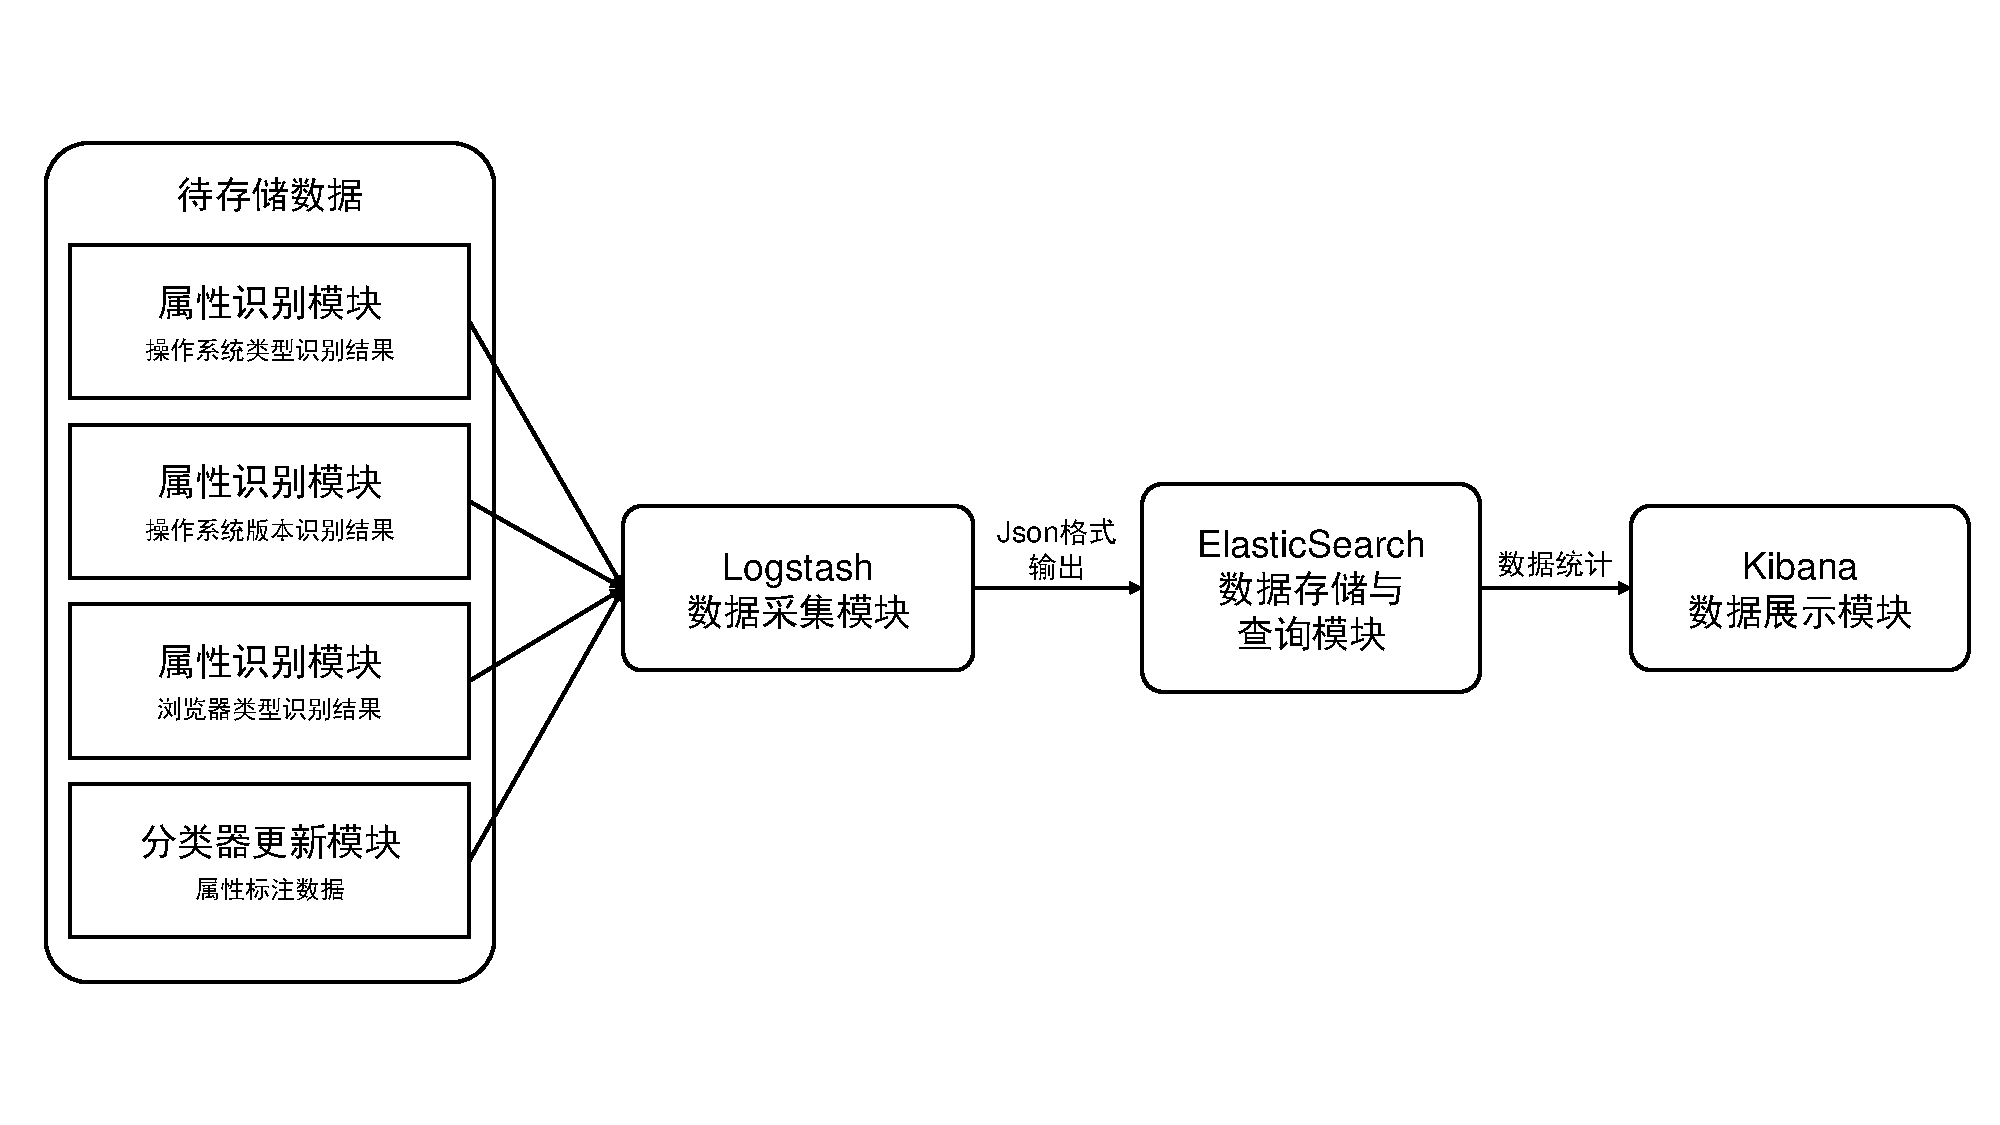
\includegraphics[width=0.9\textwidth]{数据存储}
    \bicaption{数据存储与可视化模块}{Data storage and visualization module}
\end{figure}

\section{系统测试}

\subsection{测试环境}

将本章介绍的原型系统实现后部署在某科研网络的实验环境中,环境配置如表5.1所示,操作系统为Ubuntu系统,CPU型号为Intel Xeon E5-2640,深度学习分类器采用的GPU型号为GTX 1080Ti,设备内存最大为94GB,网络中的流速均值为200MBps。在编程实现方面,流量采集模块与特征提取模块基于C语言实现,属性识别模块和分类器更新模块基于Python语言实现,数据存储和可视化模块基于ElasticSearch数据库实现。

\begin{table}[!h] 
    \bicaption{实验环境}{Lab environment}
    \centering
    \footnotesize
    \setlength{\tabcolsep}{25pt}
    \renewcommand{\arraystretch}{1}
\begin{tabular}{|c|l|}

\hline
操作系统 & Ubuntu 16.04.6 LTS \\ \hline
CPU型号 	& Intel Xeon E5-2640\\ \hline
GPU型号& GTX 1080Ti\\ \hline
内存大小& 94GB\\ \hline
网络流速 & 200MBps \\\hline

\end{tabular}
\end{table}

\subsection{系统运行性能测试}

本文在2020年1月3日到1月12日对系统进行为期十天的部署测试,观察并分析了系统在资源消耗方面和识别性能方面的表现,评估了原型系统在主机属性发现任务中的计算成本、空间成本以及识别有效性。

如表5.2所示,系统平均每天检测1465833条TLS会话,包含132075个客户端主机。在十天的运行结果中,对单核CPU的占用率峰值最高为87.4\%,内存率占用峰值最高为7.1\%,处理速度最快可以达到每分钟识别4357条会话。在GPU占用方面,基于Tensorflow实现的深度学习分类器对单核GPU的利用率最高可接近100\%。由此可见,本系统的计算复杂度较高,对内存空间的需求较小。在表5.1所示的实验条件下,系统可实现对主机属性的实时发现。

\begin{table}[!h] 
    \bicaption{系统运行性能}{System performance}
    \centering
    \footnotesize
    \setlength{\tabcolsep}{6pt}
    \renewcommand{\arraystretch}{1}
\begin{tabular}{ccccccc}
\toprule
天数 &TLS会话数目 &客户端主机数 & CPU峰值 & GPU峰值 & 内存峰值 & {\begin{tabular}[c]{@{}c@{}}吞吐量峰值\\ (样本/分钟)\end{tabular}}\\ 
\hline
1 & 1207243 & 135938  & 61.7\% & 98.8\% & 5.2\% & 3767\\
2 & 1649110 & 121809  & 87.4\% & 99.1\% &7.1\% &  4133\\
3 & 1601300 & 133736  & 76.9\% & 98.3\% &5.8\% &  3914\\
4 & 1371310 & 145284  & 50.2\% & 98.7\% &4.9\% &  3501\\
5 & 1689831 & 139410  & 51.3\% & 99.1\% &5.3\% &  3591\\
6 & 1494181 & 122342  & 67.6\% & 99.8\% &5.8\% &  3762\\
7 & 1282757 & 130111  & 81.4\% & 99.8\% &6.7\% &  4357\\
8 & 1589818 & 142170  & 70.3\% & 98.4\% & 6.1\% &  4206\\
9 & 1190328 & 122802  & 81.7\% & 99.7\% & 6.1\% &  3924\\
10 & 1582456 & 127149 & 81.2\% & 99.8\% & 6.3\% & 4008\\
均值 & 1465833 & 132075 &  70.9\% & 99.2\%& 5.9\% & 3916\\
\bottomrule
\end{tabular}
\end{table}

\subsection{分类器识别性能测试}

在系统测试过程中,本文发现,由于实时网络中的流量数据复杂多样,流量采集模块捕获的某些会话数据存在异常(缺失、噪声、不一致、冗余),无法提取有效特征,导致分类器不能有效识别其主机属性信息。

此外,由于属性识别模块目前的识别范围是有限的,只能识别主流的操作系统类型、版本以及浏览器类型。而在开放的实验网络中,可能存在识别范围之外的TLS会话数据,例如Symbian系统、BlackBerry OS系统、360浏览器、QQ浏览器等操作系统或浏览器发起的TLS会话。这些会话样本数据虽然占比非常小,但可能在一定程度上导致分类器的误识别,降低识别准确性。

为了筛选出上述问题产生的异常会话样本,本文优化了分类器的识别策略。在一般的分类器识别过程中,机器学习模型会对每个样本预测其属于某个类别的概率,然后选择概率最大的类别作为识别结果。通过深入统计分析,我们发现分类器对异常样本的类别预测概率通常都低于50\%。因此,本文假设仅当分类器的类别预测概率最大值高于50\%时,才会选择概率最大的类别作为识别结果,否则视为识别失败,即该样本不属于任何类别。

\begin{table}[!h] 
    \bicaption{分类器识别性能}{Classifier identification performance}
    \centering
    \footnotesize
    \renewcommand{\arraystretch}{1}
\begin{tabular}{ccccccc}
\toprule
\multirow{2}{*}{天数} & \multicolumn{3}{c}{识别率} & \multicolumn{3}{c}{F1分数} \\ \cline{2-7}
& 操作系统类型 & 操作系统版本 & 浏览器类型 &操作系统类型 & 操作系统版本 & 浏览器类型 \\ \hline
1 & 95.11\% & 94.13\% & 91.61\% & 96.51\% & 79.92\% & 95.14\% \\
2 & 94.25\% & 93.71\% &  91.53\% & 95.16\% & 82.79\% & 94.87\% \\
3 & 95.24\% & 94.11\% & 91.60\% & 96.47\% & 82.82\% & 94.98\% \\
4 & 93.71\% & 91.93\% & 92.33\% & 96.23\% & 82.83\% & 95.25\% \\
5 & 95.92\% & 94.27\% & 89.96\% & 96.01\% & 80.78\% & 95.54\% \\
6 & 96.30\% & 93.67\% & 92.41\% & 96.53\% & 81.13\% & 95.51\% \\
7 & 96.11\% & 95.86\% & 93.40\% & 95.90\% & 80.72\% & 96.20\% \\
8 & 91.62\% & 91.07\% & 92.42\% & 96.22\% & 82.09\% & 94.74\% \\
9 & 95.98\% & 93.24\% & 92.99\% & 96.48\% & 79.72\% & 96.22\% \\
10 & 94.42\% & 93.19\% & 91.94\% & 96.21\% & 81.14\% & 95.85\% \\
均值& 94.87\% & 93.52 \% & 92.02\%  & 96.17\% & 81.40\% & 95.43\% \\
\bottomrule
\end{tabular}
\end{table}

在如表5.3所示的分类器识别性能测试结果中,系统对操作系统类型的识别成功率均值为94.87\%,对操作系统版本的识别成功率均值为93.52\%,对浏览器类型的识别成功率均值为92.02\%。其中,系统对浏览器类型识别的成功率最低,这主要是因为实验网络中较多主机使用了识别范围之外的小众浏览器。

F1分数是模型精确度的一种指标。它同时兼顾了分类模型的精确率和召回率。从表5.3所示分类结果的F1分数来看,属性识别模块中的Stacking集成模型比第3章和第4章中介绍的所有单一模型效果都要更好,充分体现了Stacking技术的优越性。此外,系统在十天中的各方面性能变化都比较小,最大差异没有超过3\%,这一结果也证明了本系统拥有较强的稳定性和鲁棒性。

\subsection{可视化功能测试}

本文在2020年1月12日晚截取了系统的实时可视化Web页面,如图5.7所示,主要向用户展示了系统当日已识别的客户端数目,每天处理的会话数目以及各种主机属性的统计结果等。除此之外,系统还可以根据需要从数据库中快速检索并绘制更多表格和图像,方便用户对识别结果进行观察和分析。

\begin{figure}[!htbp]
    \centering
    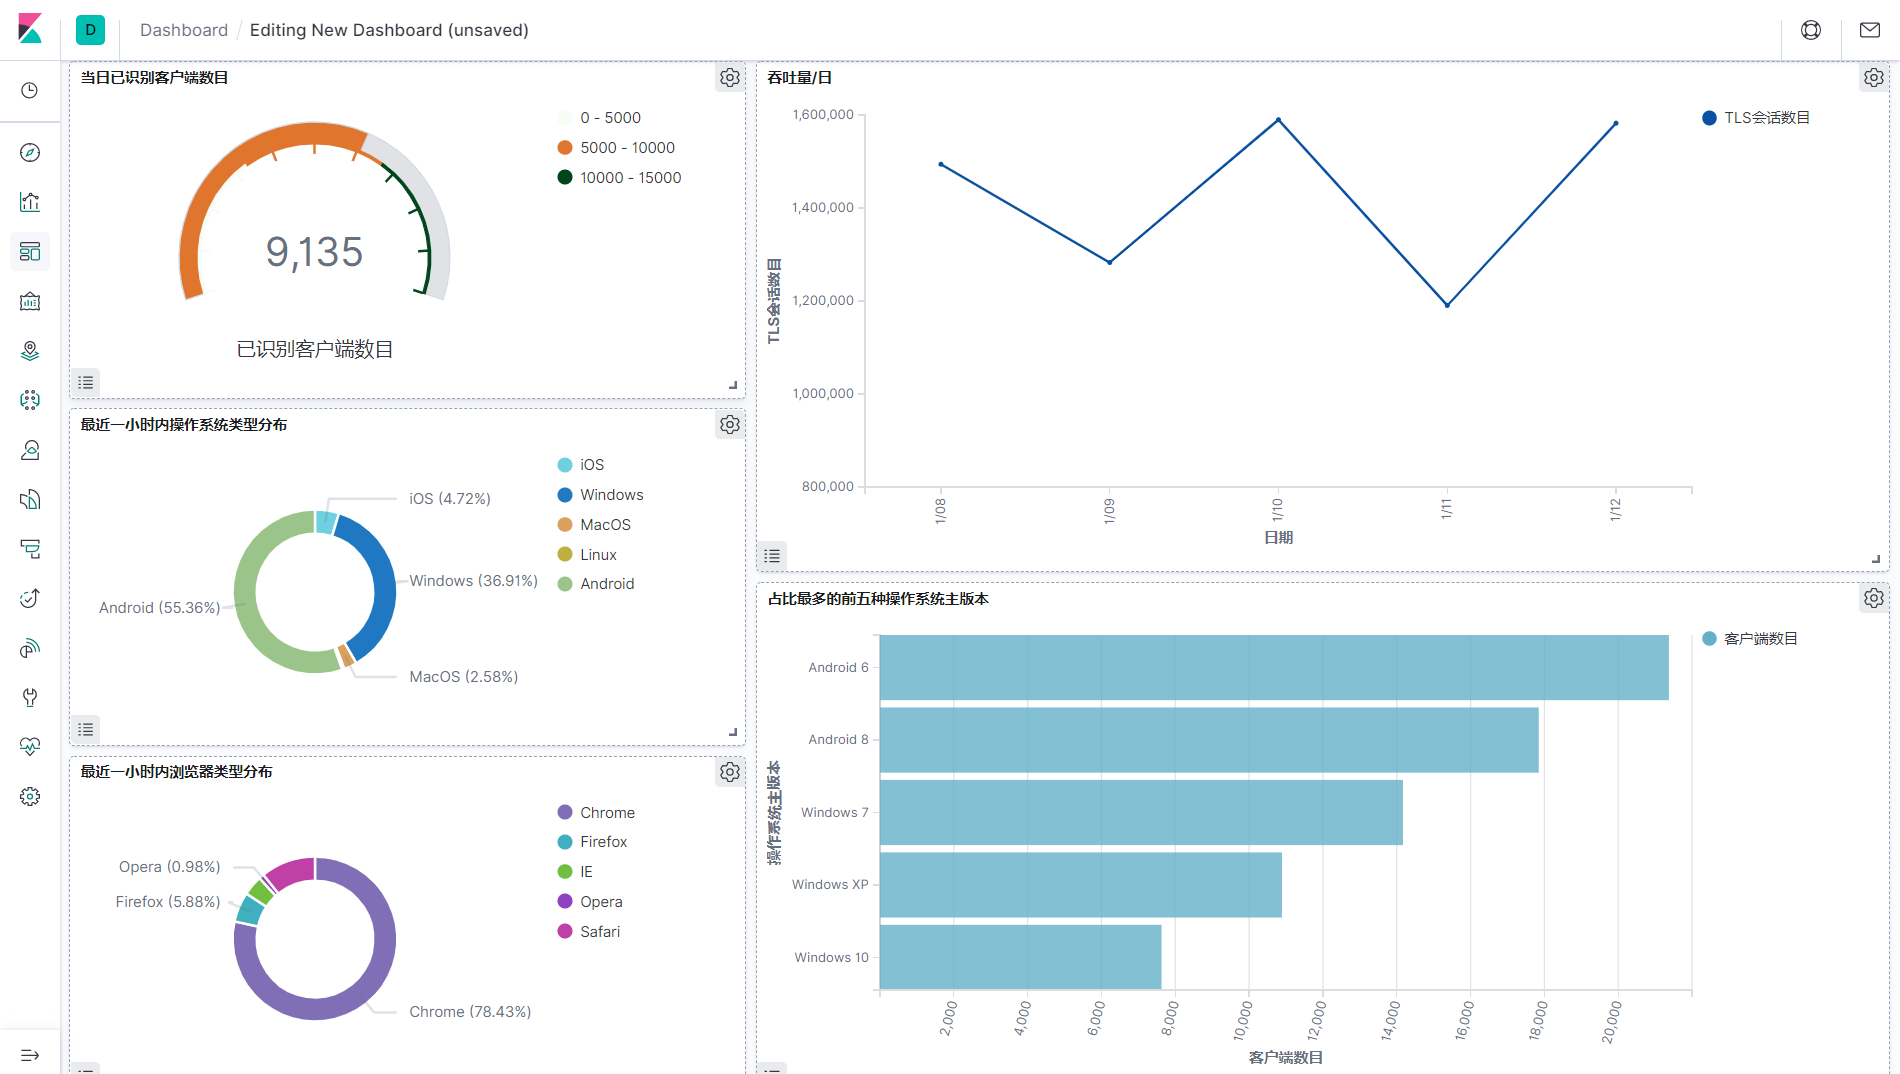
\includegraphics[width=0.8\textwidth]{可视化}
    \bicaption{可视化页面}{Visual page}
\end{figure}

\subsection{识别结果分析}

在为期十天的系统测试结果中,本系统共发现了5种操作系统类型,5种浏览器类型和22种操作系统版本,操作系统类型主要为Android、Windows、iOS、MacOS以及Linux等,版本包括上述5种操作系统的22种主版本,浏览器类型主要为Chrome、Safari、IE、Firefox以及Opera等。

在图5.8所示的操作系统类型识别结果中,Android系统和Windows系统的数量最多,共计占比约87.3\%,其次是Apple公司设计开发的iOS系统和MacOS系统,约占10\%,Linux系统的数量最少,只有2.7\%。

\begin{figure}[!h]
    \centering
    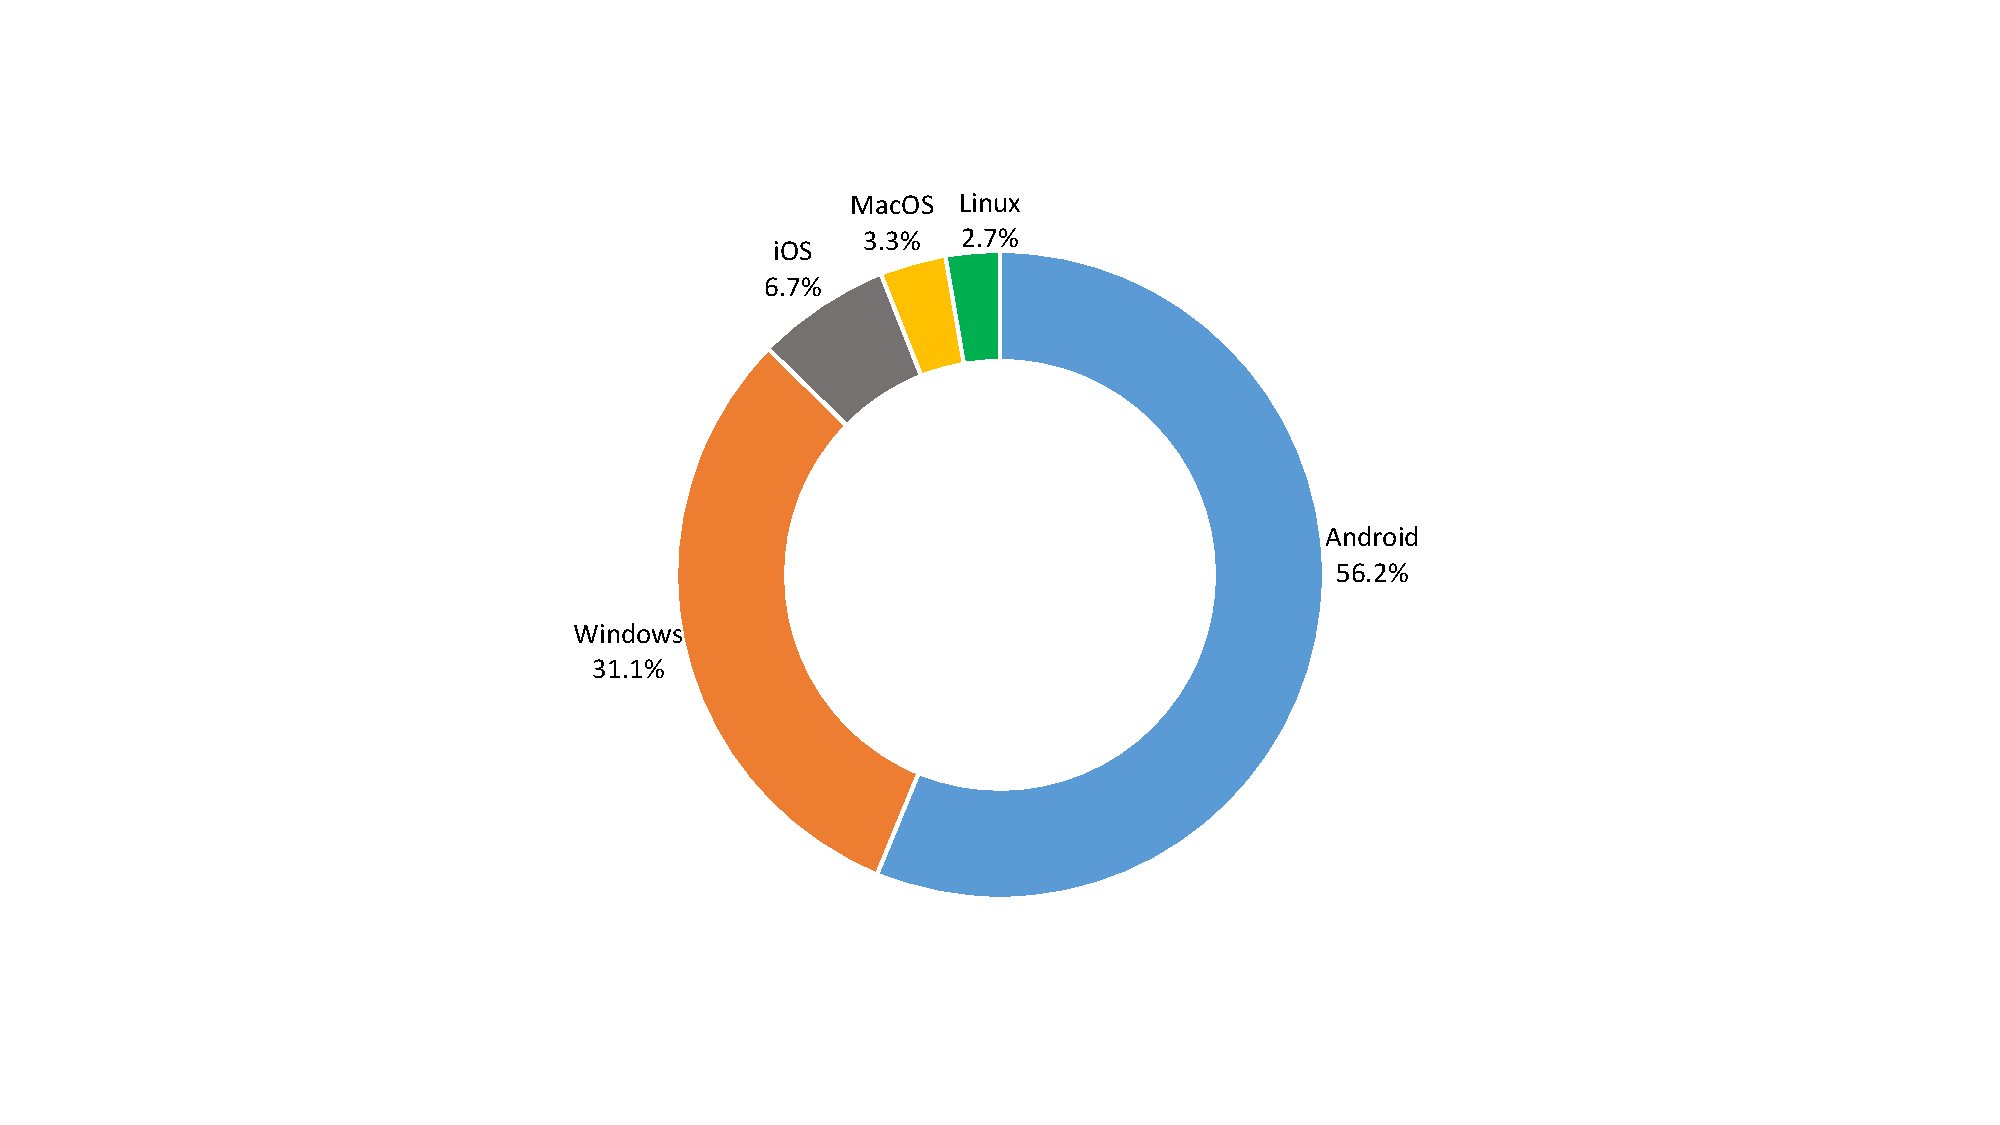
\includegraphics[width=0.59\textwidth]{os类型分布}
    \bicaption{识别结果中的操作系统类型分布}{Distribution of operating system type  in the identify ressults}
\end{figure}

在浏览器类型识别结果中,如图5.9所示,最受用户欢迎的浏览器是Chrome浏览器,占比约为70.6\%,比排名第二的Safari浏览器多出近50\%。IE浏览器作为微软公司的官方浏览器和Windows系统的默认浏览器,其使用量却非常少,仅占比约4.9\%。而经典的Firefox浏览器和Opera浏览器则更为少见,共计占比约4.8\%。

\begin{figure}[!h]
    \centering
    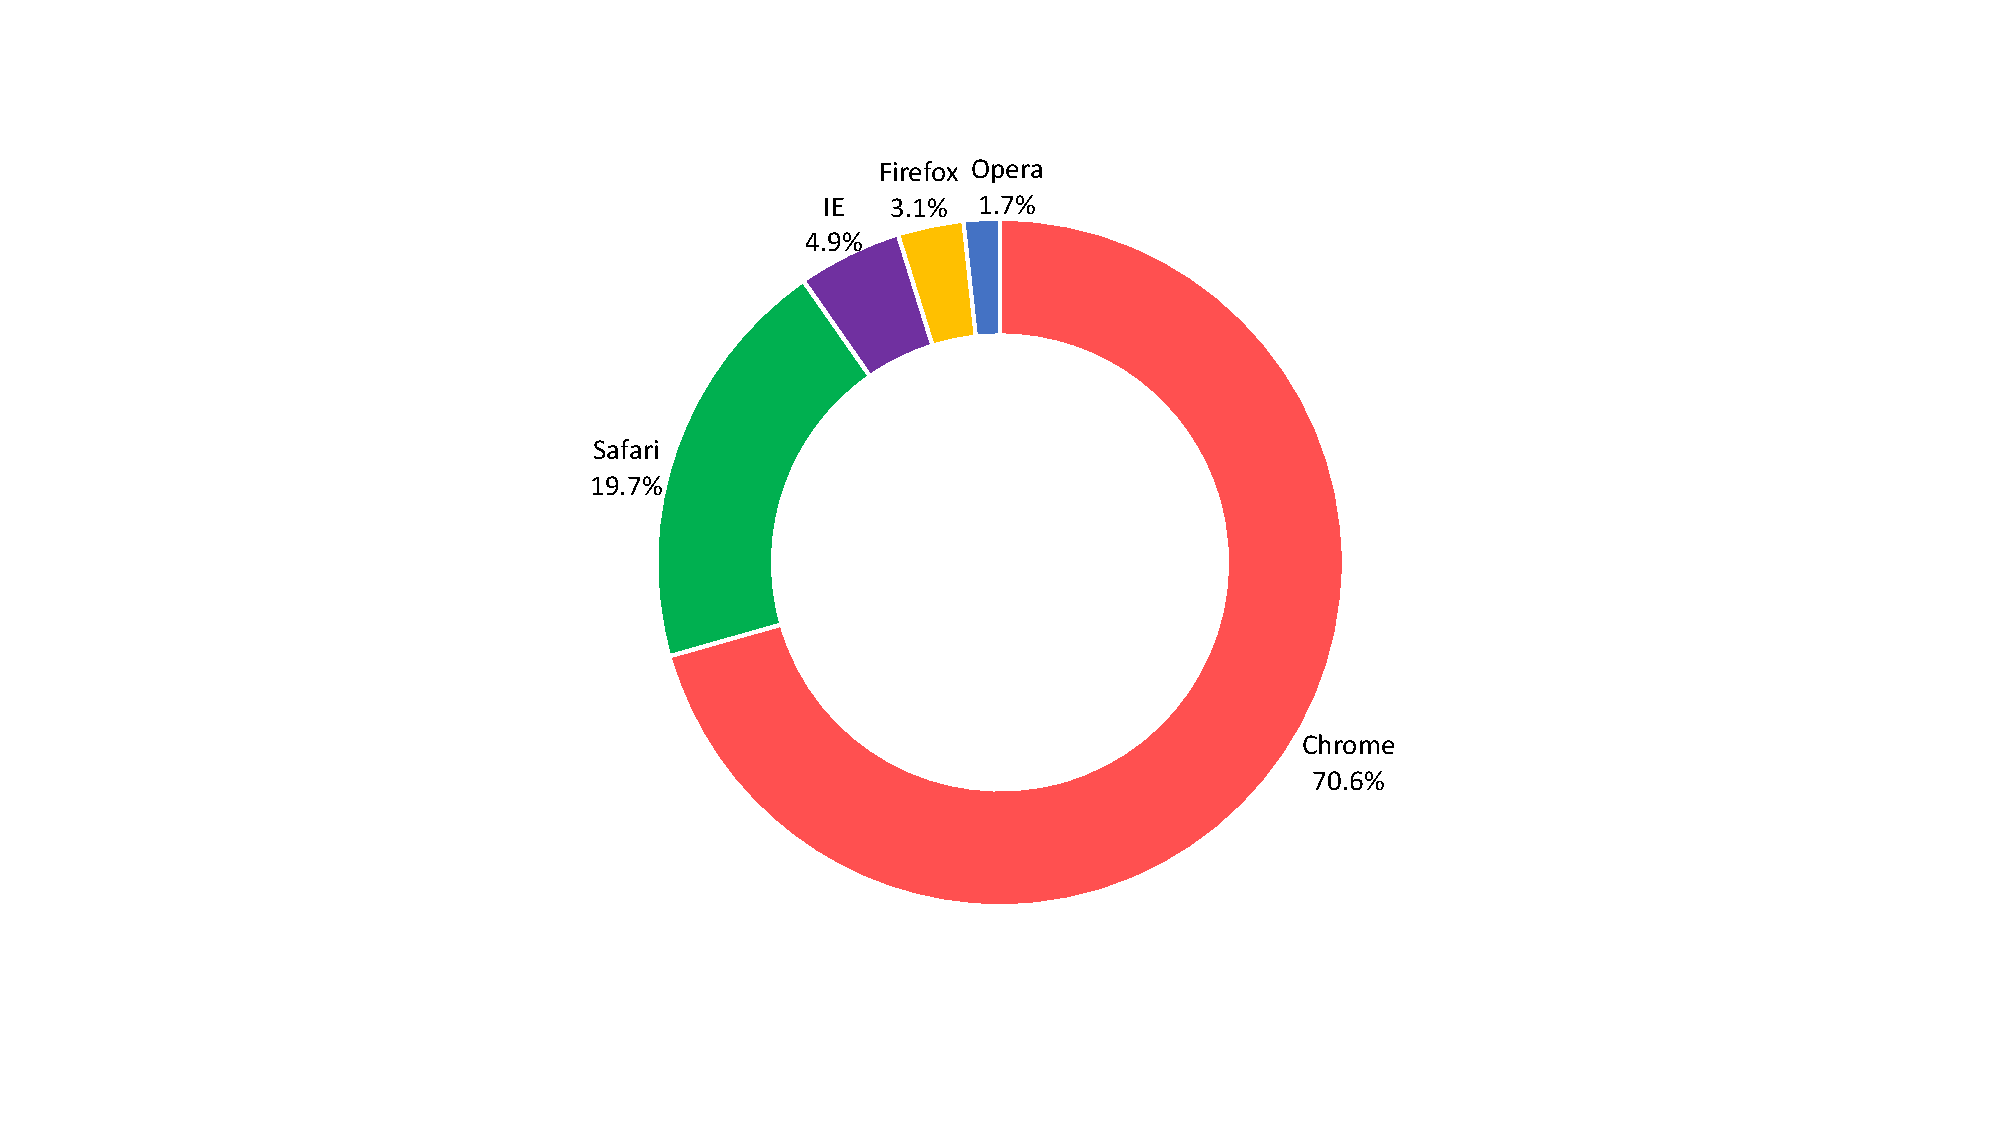
\includegraphics[width=0.55\textwidth]{bs类型分布}
    \bicaption{识别结果中的浏览器类型分布}{Distribution of browser type in the identify ressults}
\end{figure}

图5.10展示了操作系统版本的识别结果分布,从中可以发现,无论是最常见的Android系统和Windows系统,还是较为小众的iOS系统和MacOS系统,在其历史版本中,使用量最多的往往不是最新版本,而是稳定性和兼容性较好的经典版本。此外,在所有版本的系统中,Android 6、Android 8以及Windows 7系统的占比最多,共为49.5\%,
\begin{figure}[!h]
    \centering
    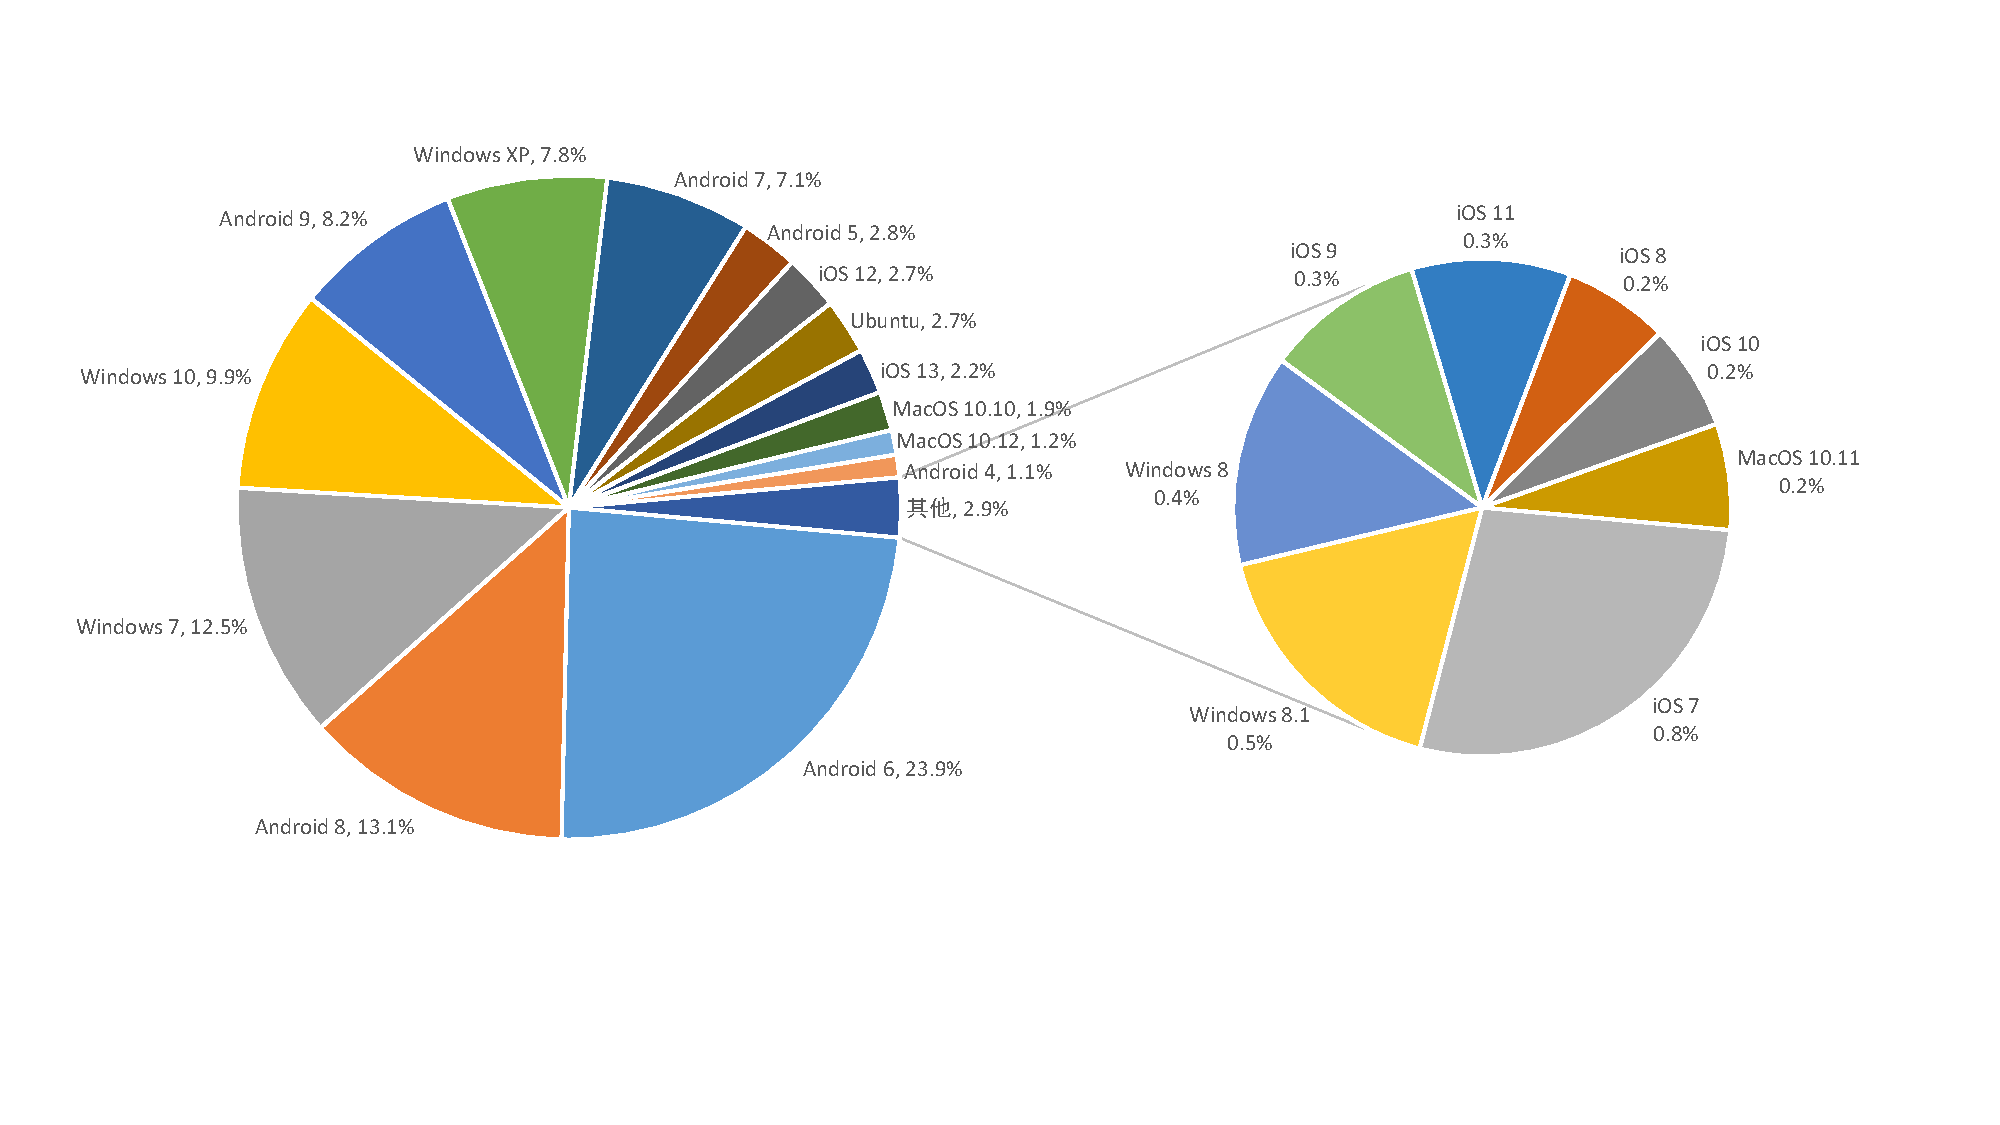
\includegraphics[width=0.9\textwidth]{os版本分布}
    \bicaption{操作系统版本分布}{Operating system Version distribution}
\end{figure}

\section{本章小结}

本章基于前文的研究成果,设计并实现了一个基于加密流量指纹的主机属性发现原型系统。本系统首先从实时网络中识别和采集HTTP流量和TLS流量,以五元组为标识将每个网络会话的所有数据包按序汇集为双向流。然后从流中提取所需特征和标签,特征主要包括协议首部字段特征、流统计特征以及流原始字节特征,标签主要为从HTTP协议首部User-Agent字段中提取出的主机属性信息。根据特征数据,系统中的Stacking集成分类器可快速、准确地识别每条TLS流的主机属性信息,同时结合标签数据,系统可完成对分类器的更新与优化。最终,基于Elasticsearch开源搜索平台,实现对识别信息的存储、查询与可视化。

通过在实时网络中部署并进行为期十天的测试,完成了对原型系统的性能评估,证明了系统具有优秀的鲁棒性和识别精度,其提供的可视化功能可以方便用户观察识别结果。
